% ### Uses XeLaTeX ### %
% ### Needs beamer-master ### %
\documentclass[aspectratio=169]{beamer} %. Aspect Ratio 16:9
\usetheme{AI2} % beamerthemeSprace.sty
% DATA FOR FOOTER
\date{2020}
\title{}
\author{}
\institute{Advanced Institute for Artificial Intelligence (AI2)}

\usetikzlibrary{calc,chains,shadows}
\usepackage{tikz}
\usepackage{subfigure}

\begin{document}    
% ####################################
% FIRST SLIDE 						:: \SliTit{<Title of the Talk>}{<Author Name>}{<Intitution>}
% SLIDE SUB-TITLE					:: \SliSubTit{<Title of the Chapter>}{<Title of the Section>}
% SLIDE WITH TITLE 					:: \SliT{<Title>}{Content}
% SLIDE NO TITLE 						:: \Sli{<Content>} 
% SLIDE DOUBLE COLUMN WITH TITLE 	:: \SliDT{<Title>}{<First Column>}{<Second Column>}
% SLIDE DOUBLE COLUMN NO TITLE 		:: \SliD{<First Column>}{<Second Column>}
% SLIDE ADVANCED WITH TITLE 			:: \SliAdvT{<Title>}{<Content>}
% SLIDE ADVANCED  NO TITLE 			:: \SliAdv{<Content>}
% SLIDE ADVANCED DOUBLE TITLE 		:: SliAdvDT{<Title>}{<First Column>}{<Second Column>}
% SLIDE ADVANCED DOUBLE NO TITLE 	:: SliAdvD{<First Column>}{<Second Column>}
% ITEMIZE 							:: \begin{itemize}  \IteOne{1st Level} \IteTwo {2nd Level} \IteThr{3rd Level} \end{itemize}
% SECTION 							:: \secx{Section} | \secxx{Sub-Section}
% COLOR BOX 						:: \blu{blue} + \red{red} + \yel{yellow} + \gre{green}
% FRAME 							:: \fra{sprace} \frab{blue} \frar{red} + \fray{yellow} + \frag{green}	
% REFERENCE						:: \refer{<doi number>}
% FIGURE 							::  \img{X}{Y}{<scale>}{Figures/.png} 
% FIGURE							:: \begin{center}\includegraphics[scale=<#>]{Figures/.png}\end{center}
% PROJECT STATUS					:: \planned\~    \started\~   \underway\~   \done\~   
% EXERCICIO							:: \Exe{<#>}{<text>}
% STACKREL							:: \underset{<down>}{<up>}
% FLUSH LEFT						:: \begin{flalign*}  & <1st equation> & \\  & <12nd equation>  & \\ \end{flalign*}
% REAL / IMAGINAY					:: \Re / \Im
% SLASH								:: \sl{} or \sl
% BOLD MATH							:: \pmb{<>}
% ####################################
%
% FIRST SLIDE :: DO NOT BREAK LINE !!!
\SliTit{Regularização para Regressão}{Advanced Institute for Artificial Intelligence}{https://advancedinstitute.ai}

% SLIDE WITH TITLE
\SliT{Regressão: Onde estamos}{
\secx{Mesmo com modelos relativamente simples, conseguimos fazer um fit bom no conjunto de treinamento}

\begin{figure}
    \centering
    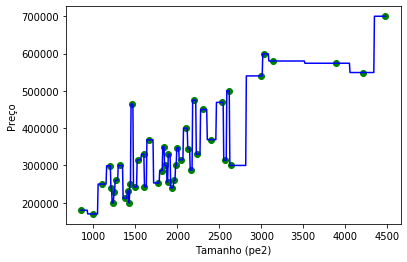
\includegraphics[width=0.5\columnwidth]{figs/fit_tree.png}
\end{figure}

}

\Sli{
    \secx{Seria mesmo?}
    \begin{itemize}
        \item Modelos complexos tem tendência a se especializarem demais ao conjunto de treinamento.
        \item Modelos que aderem perfeita e completamente aos exemplos mostrados correm risco de \textit{overfitting}
    \end{itemize}

}

\Sli{
    \secx{Mas o que teria de ruim em aderir perfeitamente aos dados?}
    \begin{itemize}
        \item \textbf{Lembre-se:} O Conjunto de treinamento não é uma representação perfeita do mundo real
        \item O objetivo principal é modelar um fenômeno através de exemplos, saber classificar apenas o conjunto de treinamento não vale de nada
    \end{itemize}

}

\Sli{
\begin{figure}
    \centering
    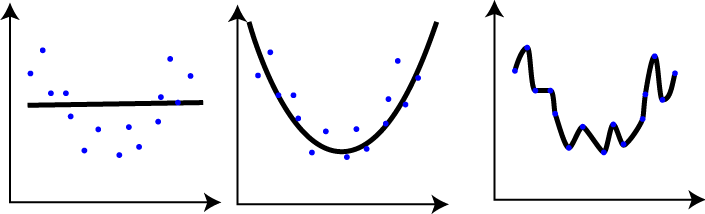
\includegraphics[width=0.6\columnwidth]{figs/under_and_overfit.png}
    \caption{(Esquerda): Underfit, (Centro): Fit, (Direita): Overfit}
\end{figure}

}

\SliT{Visualizando Overfitting}{
\secx{Como o modelo da árvore muda ao retirar alguns exemplos}

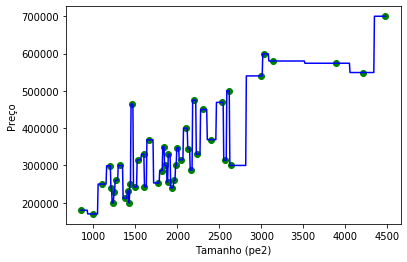
\includegraphics[width=0.45\columnwidth]{figs/fit_tree.png}
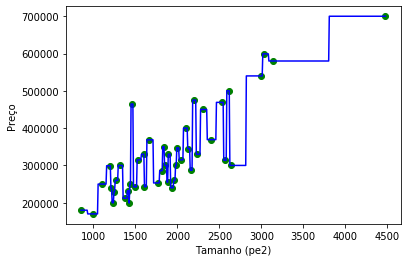
\includegraphics[width=0.45\columnwidth]{figs/fit_tree_mod.png}
}

\Sli{
\secx{Modelo linear tem sensibilidade a outliers}

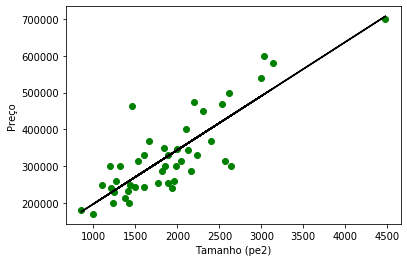
\includegraphics[width=0.45\columnwidth]{figs/fit_line.png}
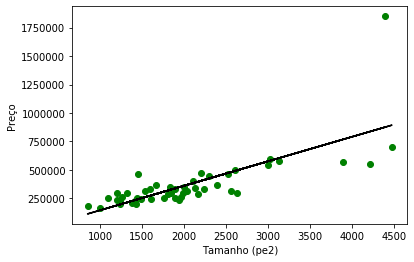
\includegraphics[width=0.45\columnwidth]{figs/fit_line_mod.png}
}

\SliT{Como saber se o modelo tem overfitting?}
{
\begin{itemize}
    \item Sempre avaliar modelos em amostras que o \textbf{modelo nunca viu}
    \item Fazer divisões em bases de treinamento e teste, possivelmente utilizando validação cruzada
\end{itemize}
}

\SliT{Estudo base Portland: Árvore}{
\secx{Base de treinamento: \textbf{$R^2 = 1.0$}}
\begin{figure}
    \centering
    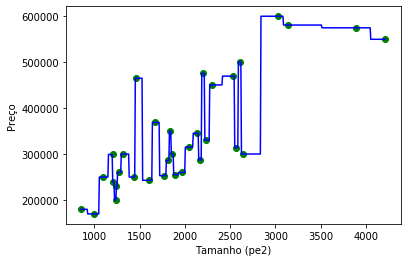
\includegraphics[width=0.45\columnwidth]{figs/portland_training.png}
\end{figure}


}

\Sli{
\secx{Base de teste: \textbf{$R^2 = 0.43$}}
\begin{figure}
    \centering
    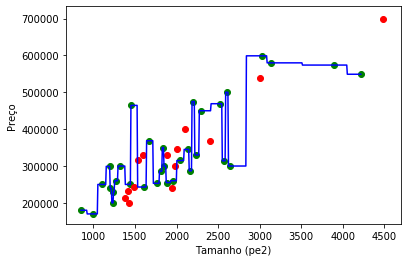
\includegraphics[width=0.45\columnwidth]{figs/portland_test.png}
\end{figure}


}


\SliT{Interpretação da base de teste}{
\secx{Métrica perfeita na base de teste significa que o modelo é perfeito?}
\begin{itemize}
    \item \textbf{Não necessariamente}: Em nenhum problema não-trivial você terá acesso à uma base de dados completamente representativa do problema
    \item Avaliar com uma base de teste \textit{alivia}, não resolve o problema
    \item Nunca haverá exemplos suficientes para modelar perfeitamente o fenômeno
\end{itemize}


}

\SliT{Dilema: Variância x Viés}{
\begin{figure}
    \centering
    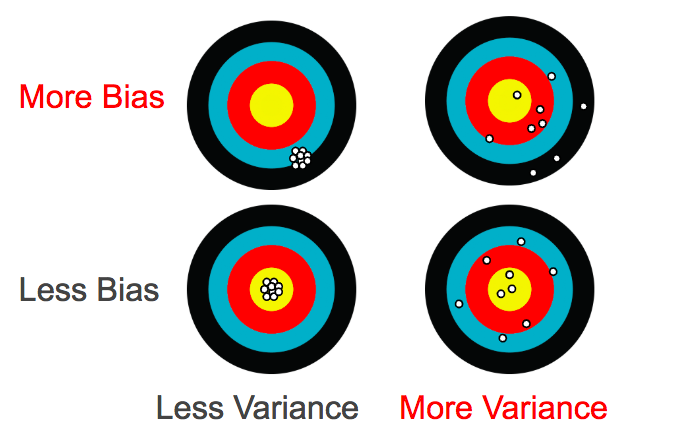
\includegraphics[width=0.6\columnwidth]{figs/variance_x_bias.png}
\end{figure}

}

\Sli{

\begin{itemize}
    \item Bias é a diferença entre a previsão média do modelo e o valor correto que estamos tentando prever. Bias alto siginifica que o modelo é simplificado demais para os dados.
    \item Variância é a variabilidade da previsão do modelo para um dado ponto de dados. O modelo com alta variação presta muita atenção aos dados de treinamento e não generaliza suficientemento para os dados que não conhece. 
\end{itemize}

}

\Sli{

\begin{itemize}
    \item Modelo muito simples com poucos parâmetros tem Bias alto e baixa variação.
    \item Modelo complexo com um grande número de parâmetros, terá alta variação e Bias baixo. 
    \item Deve-se buscar  o equilíbrio / bom sem sobreajustar e não adequar os dados.
\end{itemize}

}
 
\Sli{
\begin{itemize}
    \item Os modelos devem tentar \textbf{generalizar} além do que é observado no conjunto de treinamento.
    \item A \textbf{Regularização} tem o papel de controlar o overfitting dos classificadores.
\end{itemize}

}

\SliT{Regularização}{
\begin{itemize}
    \item Diminui a \textbf{variância} reduzindo a eficácia no aprendizado
    \item Penaliza a complexidade do modelo
    \item Quase todos os algoritmos de aprendizado possuem algum mecanismo de regularização
\end{itemize}
}

\SliT{Regressão Linear}{
\secx{Regularização L2}
\\
Busca diminuir o valor dos parâmetros da função de regressão

\begin{equation*}
    J(\theta) = \frac{1}{2n}\sum_{i=1}^{n} (y_i - (\theta_0 + \theta_1 x_i))^2 {\color{red} + \sum_{\theta_i} \frac{\lambda}{2n}\theta_i^2 }
\end{equation*}

\secx{Regularização L1}

\begin{equation*}
    J(\theta) = \frac{1}{2n}\sum_{i=1}^{n} (y_i - (\theta_0 + \theta_1 x_i))^2 {\color{red} + \sum_{\theta_i} \frac{\lambda}{2n}\theta_i}
\end{equation*}
}

\SliT{Regularização}{

Dois exemplos de procedimentos de regularização para regressão linear são:

\begin{itemize}
    \item Regressão lasso: mínimos quadrados são modificados para também minimizar a soma absoluta dos coeficientes (regularização L1).
    \item Regressão Ridge: Mínimos Quadrados são modificados para também minimizar a soma absoluta ao quadrado dos coeficientes (chamada regularização L2).
    
\end{itemize}
}

\SliT{Regularização}{


\begin{itemize}
    \item Ao utilização de um modelo de regularização leva a uma normalização do modelo.
    \item Regressão Ridge é útil quando todas as variáveis são relevantes.
    \item Regressão Lasso da mais prioridade as variáveis que impactam mais no modelo, é recomendável para casos onde a influência das variáveis não é conhecida
    
\end{itemize}
}

\Sli{
\begin{figure}
    \centering
   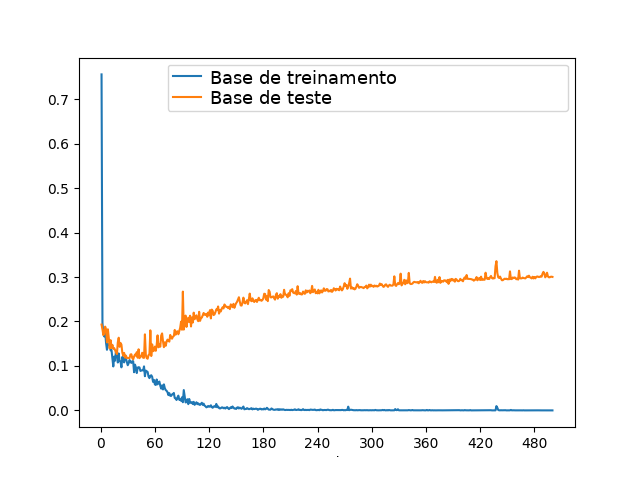
\includegraphics[width=0.45\columnwidth]{figs/overfit.png}
    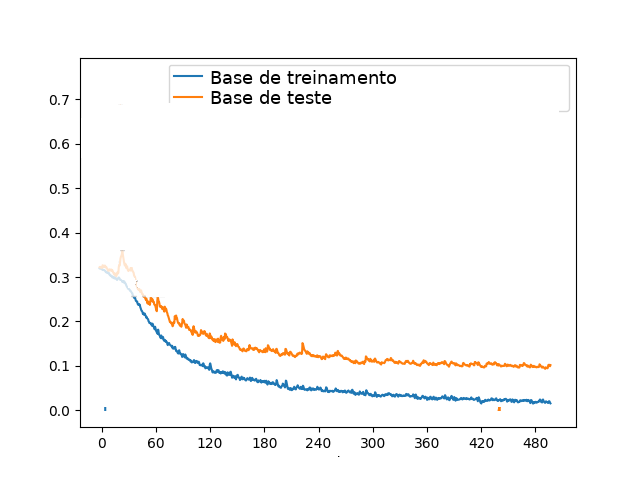
\includegraphics[width=0.45\columnwidth]{figs/regulized.png}
    \caption{(esq): Overfitting (dir): Modelo geral}
    \label{fig:my_label}
\end{figure}
    
}

\SliT{KNN}{
\begin{itemize}
    \item De certa forma, o parâmetro $K$ já funciona como um regularizador
    \item Quanto maior o $K$, mais "uniforme" a saída do regressor será
\end{itemize}
}

\SliT{Árvore de Regressão}{
\secxx{A regularização da árvore é chamada \textbf{Poda}}
\begin{itemize}
    \item A ideia principal é "podar" algumas partes da árvore que estão atrapalhando na generalização
\end{itemize}

}

\Sli{
\begin{figure}
    \centering
    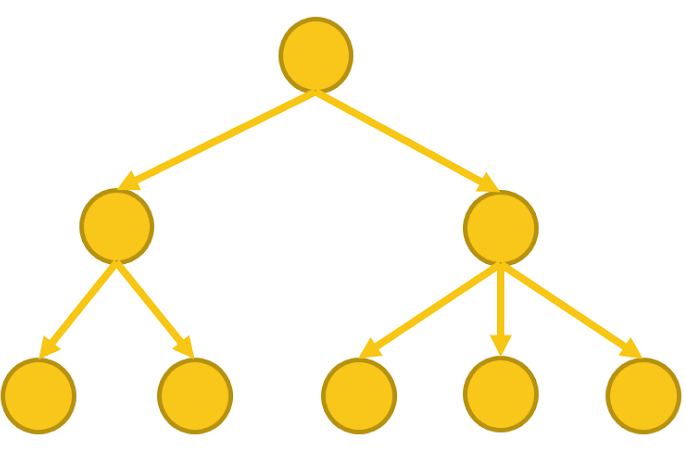
\includegraphics[width=0.6\columnwidth]{figs/arvore_para_poda.png}
\end{figure}

}

\Sli{
\begin{figure}
    \centering
    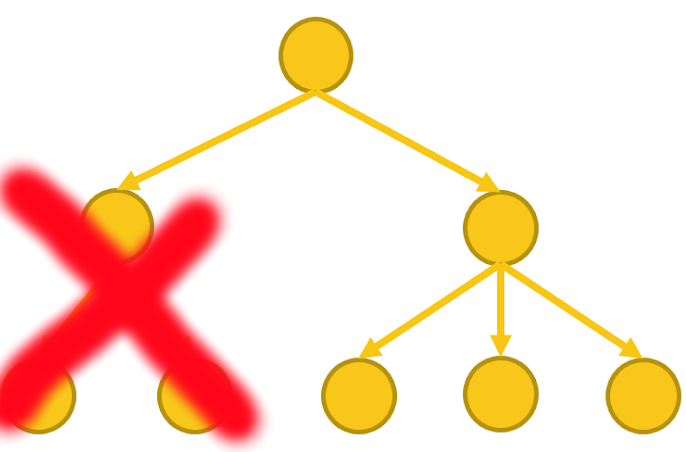
\includegraphics[width=0.6\columnwidth]{figs/arvore_podada.png}
\end{figure}

}

\Sli{
\secx{A Poda pode ser feita de muitas maneiras:}
\begin{itemize}
    \item Limitando a altura da árvore
    \item Interrompendo o crescimento da árvore após um número de nós
    \item Eliminando nós que não representem um certo número de exemplos

\end{itemize}
}



%%AQUI

\SliT{Regularização}{
\begin{itemize}
    \item A regularização limita a complexidade dos modelos
    \item Seu objetivo é dar um peso à generalização, em contraponto à otimizar a métrica de desempenho
    \item Essencial para que os modelos sejam capazes de generalizar para exemplos não vistos
\end{itemize}
}
\end{document}
